%
% points.tex
%
\renewcommand{\thisname}{Chart::Points}
\section{\thisname}
\name{\thisname}
\file{Points.pm}
\requires{Chart::Base, GD, Carp, FileHandle}
\begin{Description}
The class \thisclass creates a point chart (also called
\emph{scattergram}) where the individual data points are marked with a
symbol. (If you want lines in addition, check
\class{Chart::LinesPoints} on page~\pageref{Chart::LinesPoints}.)
\thisclass is a subclass of \class{Chart::Base}.
\end{Description}

\example
\begin{figure}[ht]
  \begin{center}
    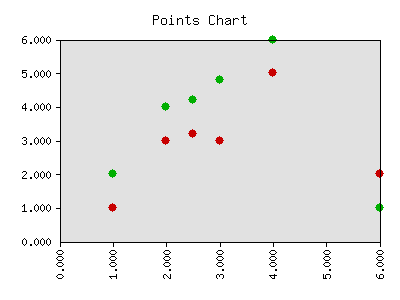
\includegraphics[scale=0.5]{points.png}
  \end{center}
  \caption{Points chart}
  \label{fig:points}
\end{figure}

\begin{verbatim}
use Chart::Points;

$g = Chart::Points->new();
$g->add_dataset(1, 4,   3, 6, 2, 2.5);  # x-coordinates
$g->add_dataset(1, 5,   3, 2, 3, 3.2);  # y-coordinates dataset 1
$g->add_dataset(2, 6, 4.8, 1, 4, 4.2);  # y-coordinates dataset 2

@hash = ('title'        => 'Points Chart',
         'xy_plot'      => 'true',
         'x_ticks'      => 'vertical',
         'legend'       => 'none',
         'sort'         => 'true',
         'precision'    => 3,
         'include_zero' => 'true',
        );

$g->set(@hash);

$g->png("Grafiken/points.png");
\end{verbatim}

\constructorblurb{\thisname}

\begin{AttrDecl}{pt\_size}
Sets the radius of the points in pixels. Default is 18.\\
The points are extended by different brush styles.
\end{AttrDecl}

\begin{AttrDecl}{brushStyle}
Define the share of the points. The share may be specified to each dataset.\\
The possible shapes of the 'points' are
\begin{itemize}
\item FilledCircle (default),
\item circle,
\item donut,
\item OpenCircle,
\item triangle,
\item upsidedownTriangle,
\item square,
\item hollowSquare,
\item OpenRectangle,
\item fatPlus,
\item Star,
\item OpenStar,
\item FilledDiamond, 
\item OpenDiamond
\end{itemize} 
To apply a different brush style to different data sets the following
example of code can be used:
\begin{verbatim}
$g->set(brushStyles => { dataset0 => 'fatPlus', dataset1 => 'hollowSquare' });
\end{verbatim}
\begin{figure}[htp]
  \begin{center}
    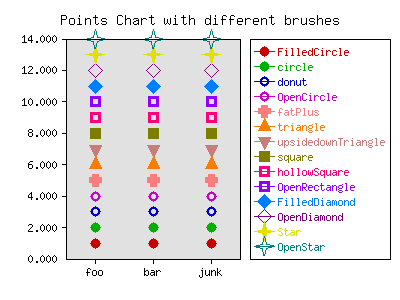
\includegraphics{brushstyles.png}
  \end{center}
  \caption{Points chart as an example for brush styles}
  \label{fig:brushStyles}
\end{figure}
\end{AttrDecl}

\begin{AttrDecl}{sort}
Sorts the data in ascending order if set to \literal{true}. Should be
set if the input data is not sorted. Defaults to \literal{false}.
\end{AttrDecl}

\attrdecl{xlabels}
\begin{AttrDecl}{xrange}
This pair of options allows arbitrary positioning of $x$ axis labels.
The two options must either both be specified or both be omitted.
\attruse{xlabels} is a reference to 2-element array. The first of the
elements is a nested (reference to an) array of strings that are the
labels. The second element is a nested (reference to an) array of
numbers that are the $x$ values at which the labels should be placed.
\attruse{xrange} is a 2-element array specifying the minimum and maximum
$x$ values on the axis. \Eg,
\begin{verbatim}
@labels = (['Jan', 'Feb', 'Mar'],
           [10,    40,    70   ]);
$chart->set(xlabels => \bs @labels,
            xrange  => [0, 100]
           );
\end{verbatim}
\end{AttrDecl}

\begin{AttrDecl}{xy\_plot}
Forces \thisclass to plot a $x$--$y$ graph if set to \literal{true},
\ie, to treat the $x$ axis as numeric. Very useful for plots of
mathematical functions. Defaults to \literal{false}.
\end{AttrDecl}

\begin{AttrDecl}{y\_axes}
Tells \thisclass where to place the $y$ axis. Valid
values are \literal{left}, \literal{right} and \literal{both}. Defaults
to \literal{left}.
\end{AttrDecl}
